\chapter{Literature Review: Survey of Related Previous Work - Overview of Wireless Sensor Network Technology}

\section{Methodology}

A search of literature was conducted using IEEE database to locate relevant literature relating to wireless applications in operating theatre. As the number of studies of this field is relatively new and limited, the search was broadened to include reviews of studies on various existing health monitoring ICT applications and not limited to only in the operating theatre. An online search of grey literature using Google was also conducted to diversify our findings. 

The review of literature identified a number of areas where wireless technologies is highlighted in usage in the healthcare industry. Reviews have been conducted with focus on current available options, security and safety, existing wireless sensors as well as data prioritization protocols. 

\section{Introduction}

Sensors networks and wireless transmission have become the trend in the electrical and electronics fields as Internet-of-Things is starting to be the norm. One of the major role of sensors now is in the biomedical field. With the help of wireless sensor network, patient monitoring and care have becoming more advanced and easier. In the operating theatre, a range of wireless technologies have been utilized today, mainly using WiFi or Bluetooth in transmitting data from monitors to slave screens. 

Wireless Electrocardiogram(ECG) monitors are also already available, where data is transferred wireless from the electrode to the monitors directly \cite{lit1}. Similarly, there are also existing wireless sensors for blood pressure by MEMSCAP Wireless Solutions which transmits information from invasive blood pressure monitor to the display wirelessly \cite{lit2}.  

Wireless transmissions in hospitals can be achieved through several different bandwidths, which can be seen in Table \ref{literaturereview1} below. Range, power, speed is among factors that are mainly considered when selecting an appropriate wireless technology to be used. However, it is noted that as both WLAN and Bluetooth are operating in the same frequency band at 2.4-2.48Ghz, throughput of data is decreased when both are used in coexistence. WLAN is used in hospital extensively and this may be a significant issue to design a system utilizing Bluetooth \cite{lit3}. 

\begin{figure}[H]
	\centering
	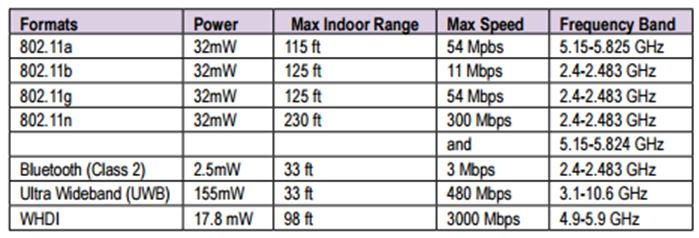
\includegraphics[width=\linewidth]{lit1.jpg}
	\caption{citeeeeeeeeeeeeeeeeeeeeee\cite{hall2015guyton}}
	\label{literaturereview1}
\end{figure}

\section{Wireless in Anaesthesia}

In the context of operating room, technical advances over the past decade have contributed to progress in anaesthesia safety. Improved patient monitoring, as well as increased usage of sensor system has introduced a new problem into practice, with great number of cables which makes care and nursing of patient difficult \cite{lit3}. 

Conventionally, sensors are wired to ensure uninterrupted monitoring of physiological variables. The use of wireless sensors will reduce the number of wires attached to the patients, easing transport and ambulation of patient in an intensive care environment \cite{lit2}. 

\section{Benefits}

There are many benefits associated with the use of wireless systems to measure vital signs in the operating theatre. First, the clutter of cables can be significantly reduced. The risk of contamination will also decrease as cables are often exposed to contamination and not easily cleaned before repeat exposure to a sterile field. In the long run, there will also be significant cost reductions associated to operating room renovations. Monitors are frequently damaged when operating room staff are required to connect and disconnect cables on a regular basis. The wear and tear of cables will also require replacement from time to time. Using wireless solutions will eliminate the need for cables completely. 

\begin{figure}[H]
	\centering
	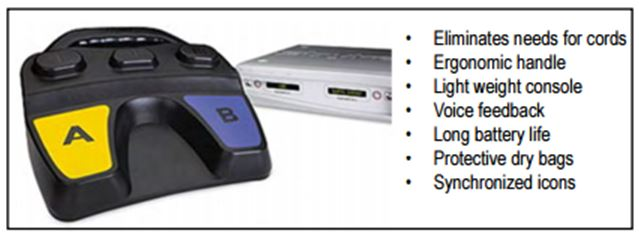
\includegraphics[width=0.7\linewidth]{lit2.jpg}
	\caption{Benefits of Wireless Monitoring Systems \cite{lit1}}
	\label{literaturereview2}
\end{figure}

For example, a wireless footswitch has been designed \cite{lit1} and this eliminates the need for cords to be draped around or placed on floor under the sterile field. It can also connect to the receiver simply and easily used by the operating room staff. This improves efficiencies, eliminate cables and obstacles reducing operating room hazards and improves the turnover rate of the operation room. 

\section{Challenges}

One of the main challenges associated with wireless monitoring systems would be security breach. It is a valid concern of someone snooping on data that is transmitted wirelessly. Adequate security and encryption have to be incorporated before it can be used in OR where a disruption of vital signs will be fatal. In the design of wireless antenna associated with the sensors, it is essential to ensure that consistent performance is achieved to avoid risk of affecting wireless range and quality of the wireless signal.  

Furthermore, interference may be a prevalent issue in wireless systems, especially when there are multiple different forms of communications existing at the same time. For example, the use of 2.4Ghz band can be crowded by WiFi and other RF traffic, which may result in noise in the signals. Using wireless technologies will also increase significant costs to the development and maintenance of the medical devices. 

\section{Priority Queueing Models}

As in our proposed model, there will be multiple sensors, namely EEG, ECG PPG etc. that are integrated into one transmission, a priority queueing model will need to be devised to ensure important vital signs data are prioritized when bandwidth / throughput is limited at certain stages of transmission. An appropriate queuing models are implemented to improve performance parameters for priority queueing, delay and server utilization time. In a study conducted by The NorthCap University \cite{lit4} indicate that using M/G/1 Or M/G/N queueing models will have better performance depending on the expected number of incoming packets. An extract of the results is shown below, serving as a reference to our queueing model. 

\begin{figure}[H]
	\centering
	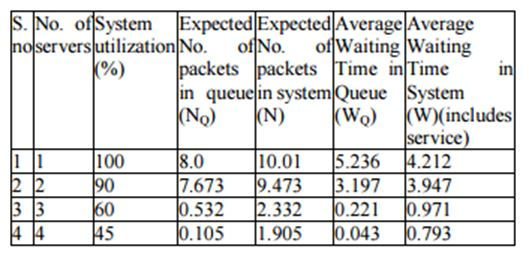
\includegraphics[width=0.7\linewidth]{lit3.jpg}
	\caption{Result for M/G/1 and M/G/N queueing models for the proposed scenario \cite{lit4}}
	\label{literaturereview3}
\end{figure}

\section{Case Studies}

There have been several successful studies that wirelessly monitors independent parameters but not all in the same package. For instance, in a project done in the University of Rhode Island \cite{lit3}, a smart wristband has been made to allow data transmission via bluetooth technology, which is able to send out BPM over standardized GATT Heart Rate Service that will calculate and output several metrics such as control point, heart rate etc. 

Wireless system that remotely monitors patient’s oxygen saturation (\%SPO2), pulse oximetry has also been devised \cite{lit5} In this project, researches have been able to transfer vital signs monitored by pulse oximeter via IEEE 902.15.4 to a wireless sensor network for storage and display. A preliminary evaluation of the proposed system indicates that it is medically satisfactory in terms of accuracy of data, validating the use of WLAN as a primary form of wireless networks. 

Case studies on Zigbee has also been done in India \cite{lit6}. By using Zigbee to monitor body temperature and heart rate, the team has managed to transmit vital parameters from body to all wirelessly connected computer. Zigbee was chosen due to convenience and cost effectiveness. However, the prototype has managed to send signals at 1Hz frequency and its power consumption is minimal. The downside is that the signal transmitted is susceptible to noise. Proof of concept of utilizing Zigbee has been established, but with limited throughput, it will not be sufficient for the arrays of data that will be transmitted in our project. 
 
With the emergence of 3D printed technology, it is possible to integrate it to design a scalable wireless monitoring system. A portable wireless systems measuring key metabolites in intensive care monitoring, using a 3d-printed case with sensing devices and integration of PCB with biosensors have been made in 2015, with successful implementation at its trials \cite{lit7}. The biosensors will then transmit its measurements via Bluetooth module to mobile Android interface. This indicate the possibility of using Android system as a universal display instead of individual displays for each of the separate sensors. 

Another solution that have been devised is to connect a dongle with wireless serial capability to convert serial data from some medical sensors to android devices such as smartphones for monitoring \cite{lit8}. This can be expanded to slave monitor, or even smart glasses in future novel applications. The use of smart devices as a platform to converge information of different sensors can also be used to recognize past trends to predict future trends, presenting a functionality of smart alarm. However, this approach do not solve the fundamental issue of Spaghetti Syndrome, but serves as a good design reference for setup of slave monitors in the Operating Room.

\section{Analysis of Existing Systems}

There are several biomedical wireless systems that have been devised for research purposes, and will be listed for comparison and benchmarking for our project. 

\subsection{Consideration of e-Health Sensor by Cooking Hacks (Libelium)}

The first would be the e-Health sensor shield, which is an interface with Arduino and Raspberry Pi to perform up to monitoring 10 different vital signs, including but not limited to SPO2, ECG, temperature, pulse etc \cite{lit9}.

\begin{figure}[H]
	\centering
	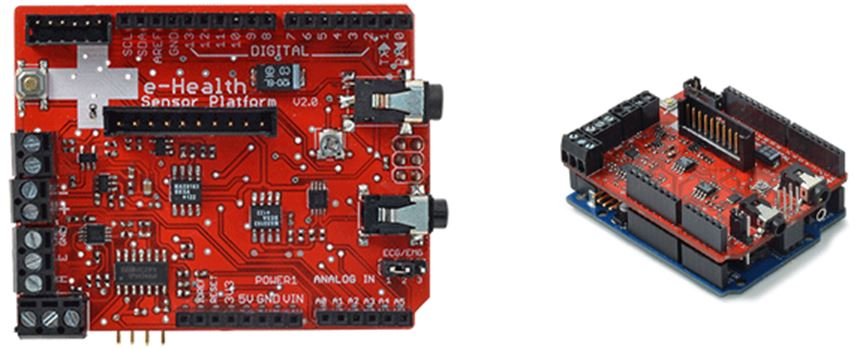
\includegraphics[width=0.7\linewidth]{lit4.jpg}
	\caption{e-Health Sensor Shield \cite{lit9}}
	\label{literaturereview4}
\end{figure}

This system is able to monitor the real time state of the patient to get sensitive data which can be subsequently used for analysis. Biometric information gather can be used to send wirelessly via multiple channel options: WiFi, 3G, GPRS, Bluetooth, 802.15.4 and Zigbee depending on application. However, this platform is designed to allow user to develop new products, i.e. an open source project to test different sensors and is not to be used in a professional medical context. 

A key takeaway from this product is the use of AES 128 for Zigbee transmission and use of WPA 2 protocol for Wifi transmission. This is important as medical data will require to be completely secure especially in the Operating Room, as a mishap in monitoring may result in fatalities.

\subsection{Consideration of BioNomadix Wireless Wearable Physiology by Biopac Systems}

Another existing system would be Bionomadix wireless wearable physiology from Biopac Systems. This is a system they are currently researching on and has developed their own platform where each BioNomadix modules can interface to \cite{lit10}. 

Each of the vital signs monitor(e.g. EEG, ECG) has separate transmitter and receiver, which makes the overall system to be bulky and harder to setup in a operating room. Contary to that, our design will allow integration of all sensors to one data transmission point, which reduces the total number of devices required for the same functionality. 

\begin{figure}[H]
	\centering
	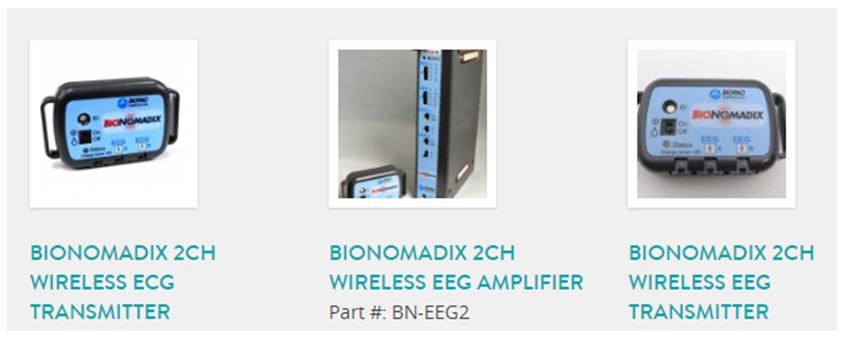
\includegraphics[width=\linewidth]{lit5.jpg}
	\caption{Sample of BioNomadix Separate Vital Sign Monitor \cite{lit10}}
	\label{literaturereview5}
\end{figure}






\section{Wireless Sensor Networks}

In line with the expansion of Internet of Things, this project is able to incorporate the idea of smart and ubiquitous connections between devices \cite{gubbi2013internet}.

\section{Body Area Networks}



\section{WiFi}

\section{Bluetooth}

\section{Zigbee}
